\section{User Evaluation}
\label{sec:user_evaluation}

As said in the introduction of this chapter, this section deals with the user 
evaluation. In order to make a proper comparison between the presented systems 
several users have been guided through a demonstration of AdaptUI and a 
comparison with Imhotep. Besides, they have been questioned according to the 
\ac{sus} guidelines.

\subsection{The \ac{sus} Questionnaire}
\label{sec:sus}
The \ac{sus}~\citep{sus}
is a 10-item questionnaire developed by John Brooke in 1986 which gives an
overview of satisfaction of users with software. Originally, it was conceived
as a ``quick and dirty'' scale to collect the usability feedback from using
systems similar to VT100 Terminal applications (see the \ac{dec} VT100 video
terminal in Figure~\ref{fig:vt100}).

\begin{figure}
\centering
\includegraphics[width=0.50\textwidth]{vt100.pdf}
\caption{The \ac{dec} VT100 video terminal, introduced in August 1978~\citep{vt100}.}
\label{fig:vt100}
\end{figure}

One of the \ac{sus} questionnaire main characteristics is its ability to collect
usability feedback through a 10 item questionnaire with 5 response options: 

\begin{enumerate}
 \item I think that I would like to use this system frequently.
 \item I found the system unnecessarily complex.
 \item I thought the system was easy to use.
 \item I think that I would need the support of a technical person to be able to
 use this system.
 \item I found the various functions in this system were well integrated.
 \item I thought there was too much inconsistency in this system.
 \item I would imagine that most people would learn to use this system very
 quickly.
 \item I found the system very cumbersome to use.
 \item I felt very confident using the system.
 \item I needed to learn a lot of things before I could get going with this
 system.
\end{enumerate}

To measure the resulting responses from the users, the formula described below
is applied: 

\begin{itemize}
 \item For odd items: subtract one from the user response.
 \item For even-numbered items: subtract the user responses from 5.
 \item This scales all values from 0 to 4 (with four being the most positive 
  response).
 \item Add up the converted responses for each user and multiply that total by 
  2.5. 
 \item This converts the range of possible values from 0 to 100 instead of from
 0 to 40.
\end{itemize}

Thus, a figure between 0 and 100 is obtained, indicating the percentage of 
acceptance of the corresponding evaluated system. 
Figure~\ref{fig:sus_responses_example} shows an example of the \ac{sus} 
questionnaire format. Besides, Table~\ref{tbl:sus_results} shows an example of 
a completed \ac{sus} questionnaire evaluating a generic system. 

\begin{figure}
\centering
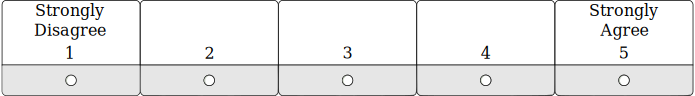
\includegraphics[width=0.65\textwidth]{sus_responses_example.pdf}
\caption{The \ac{sus} response format~\citep{vt100}.}
\label{fig:sus_responses_example}
\end{figure}


\begin{table}
 \caption{Example of a completed \ac{sus} questionnaire. Total score = 22;
 \ac{sus} Score = 22 * 22.5 = 55}
 \label{tbl:sus_results}
 \footnotesize
 \centering
\begin{tabular}{l c c c c c c}
  & \multicolumn{5}{c}{}\\
  & \begin{rotate}{60}\textbf{Disagree}\end{rotate} & & & & 
\begin{rotate}{60}\textbf{Agree}\end{rotate} \\
  \footnotesize
  1. I think that I would like to use this system frequently. 	& {\huge 
\Square} & {\huge \Square} & {\huge \Square} & {\huge \Square} & {\huge 
\CheckedBox}\\
  2. I found the system unnecessarily complex.& {\huge \Square} & {\huge 
\Square} & {\huge \Square} & {\huge \CheckedBox} & {\huge \Square}\\
  3. I thought the system was easy to use.& {\huge \Square} & {\huge 
\CheckedBox} & {\huge \Square} & {\huge \Square} & {\huge \Square}\\
  4. I think that I would need the support of a technical & {\huge \CheckedBox} 
& {\huge \Square} & {\huge \Square} & {\huge \Square} & {\huge \Square}\\
  person to be able to use this system. \\
  5. I found the various functions in this system were well & {\huge \Square} & 
{\huge \CheckedBox} & {\huge \Square} & {\huge \Square} & {\huge \Square}\\
  integrated. \\
  6. I thought there was too much inconsistency in this system.& {\huge \Square} 
& {\huge \Square} & {\huge \CheckedBox} & {\huge \Square} & {\huge \Square}\\
  7. I would imagine that most people would learn to use & {\huge \Square} & 
{\huge \CheckedBox} & {\huge \Square} & {\huge \Square} & {\huge \Square}\\
  this system very quickly. \\
  8. I found the system very cumbersome to use.& {\huge \Square} & {\huge 
\Square} & {\huge \Square} & {\huge \CheckedBox} & {\huge \Square}\\
  9. I felt very confident using the system.& {\huge \Square} & {\huge \Square} 
& {\huge \Square} & {\huge \Square} & {\huge \CheckedBox}\\
  10. I needed to learn a lot of things before I & {\huge \Square} & {\huge 
\Square} & {\huge \CheckedBox} & {\huge \Square} & {\huge \Square}\\
  could get going with this system. \\
\end{tabular}
\end{table}

Although there are other interesting questionnaires (i.e., \ac{sumi}~\citep{sumi},
\ac{mumms}~\citep{mumms}, \ac{quis}~\citep{quis}, and so on), the \ac{sus} 
questionnaire has become an industry standard with references in over 600 
publications~\citep{measuringusability}.

For this evaluation, and along with the \ac{sus} questionnaire, several extra 
questions have been added. The purpose of these questions is to segment the 
whole users set into different subsets of users under similar conditions. Thus, 
three extra classifications have been performed following the following 
criteria:

\begin{itemize}
  \item \textit{By age}. The users of AdaptUI might encounter different difficulties when
  dealing with the adaptation platform. For example, users older than 65 may not
  be used to using smart devices or touching screens. As shown through the 
  following charts, age and technology experience are related. To be aware of
  this issue an age based classification has been performed. The subgroups for
  this age classification are:
  \begin{itemize}
    \item Users aged under 20 years old ($x <$ 20)\footnote{The $x$ represents
    the age of the user. In this case the $x$ is also shown in the following 
charts
    during this section in the Legend.}.
    \item Users aged between 20 and 35 years old (20 $\leq x < $35).
    \item Users aged between 35 and 50 years old (35 $\leq x <$ 50).
    \item Users aged between 50 and 65 years old (50 $\leq x <$ 65).
    \item Users aged over 65 years old ($x >$ 65).
  \end{itemize}

  \item \textit{By experience with technology}. As it might happen with age, the 
  technology experience of the users might result into different usability 
  experiences when using AdaptUI. Touching screens, smart devices, or even 
  technical computer related instructions may be complex depending on the user 
  experience. Hence, a simple classification considering this problem is made 
  with the following criteria:
  
  \begin{itemize}
    \item \textit{Low}, which indicates a user who is not very familiar with 
    technology. This kind of users require non technical further explanations of 
    the AdaptUI features, purpose and characteristics. Besides, several \ac{sus} 
    questions might trouble these users. Thus, it is desirable to accompany them 
    through the \ac{sus} process.
  
    \item \textit{Medium}, which means that the user usually interacts with 
    technology and understands the most common interaction processes and technical 
    vocabulary. Nevertheless, too technical instructions and features might 
    confuse them.
    
    \item \textit{High}, which characterizes those users who have high level 
    technical knowledge due to their jobs, hobbies, age, and so forth. These 
    users do not require extra explanations or guidelines.
  \end{itemize}
  
  \item \textit{By disability}. Users are asked if they sense that they might 
  suffer from visual or hearing disabilities. Problems when dealing with devices 
  under certain context conditions are included. On the contrary, no specific 
  visual or hearing disability is concreted. The idea is to capture the feeling 
  of the users when manipulating devices under certain conditions (due to context 
  or due to their own capabilities).
\end{itemize}

Hence, before beginning with the \ac{sus} questionnaire, the following 4 questions
are presented, allowing users to select the corresponding responses through
several combo boxes:

\begin{enumerate}[label=\alph*)]
  \item Please select your age within the following ranges.
  \item Which would you say is your experience level with technology?
  \item Do you feel that, sometimes, you cannot use your mobile device as you
  would like due to a temporary or enduring visual problem? This problem might
  be caused by physiological or context conditions.
  \item Do you feel that, sometimes, you cannot use your mobile device as you
  would like due to a temporary or enduring hearing problem? This problem might
  be caused by physiological or context conditions.
\end{enumerate}

Besides, after these and the \ac{sus} questions two extra questions are presented
seeking developers feedback. The responses are requested through several check 
boxes:

\begin{enumerate}[label=\alph*)]
  \item I am a software developer and I usually work with user interfaces.
  \item Considering that I am a developer, I find the AdaptUI \ac{api} very
  helpful to ease the adaptation of user interfaces.
\end{enumerate}


\subsection{Discussion}
\label{sec:user_evaluation_discussion}

After using AdaptUI and checking its adaptation capabilities, users have been 
asked to complete the \ac{sus} questionnaire with the mentioned extra questions. 
This test has been completed by a total of 30 users. Classified into different 
groups regarding their age, technology experience and temporary or enduring 
disabilities the obtained results are explained in the following lines illustrated 
with several figures and charts.

First, without considering any of the cited classification criteria, the usability 
results regarding the AdaptUI adaptation system is illustrated through 
Figure~\ref{fig:sus_responses}. This figure shows that the 63,3\% of the users
punctuated AdaptUI with over 70 within the \ac{sus} scale. On the contrary, 
approximately 30\% of the users find its usability between 50 and 70 points.

\begin{figure}
\centering
\includegraphics[width=0.50\textwidth]{sus_responses.pdf}
\caption{The \ac{sus} responses.}
\label{fig:sus_responses}
\end{figure}

Next, the cited criteria regarding age, technology experience and possible
disabilities result in the following bar charts. The Figure~\ref{fig:sus_age}
illustrates the differences regarding the \ac{sus} results taking into account the
users' ages. In this chart, it is shown how users between 20 and 35 years old
are the ones who mostly support the AdaptUI usability results. 36,66\% of
these users consider that the usability of AdaptUI is over 70 in the \ac{sus} scale.

\begin{figure}
\centering
\includegraphics[width=0.80\textwidth]{sus_ages.pdf}
\caption{The \ac{sus} responses taking into account the age range of the users.}
\label{fig:sus_age}
\end{figure}

Along with the age, usually the experience with technology is directly related.
To have this into account, Figure~\ref{fig:sus_experience} illustrates the
resulting differences encountered after analysing the responses given to the \ac{sus}
questionnaire. As shown, users with \textit{high} technology experience 
result into bigger usability results, reaching a final result of 40\% of 
users punctuating AdaptUI over 70 points in the \ac{sus} scale. On the opposite side 
there are those users who lack technology experience. 20\% of these 
users gave less than 70 points. 

\begin{figure}
\centering
\includegraphics[width=0.80\textwidth]{sus_experience.pdf}
\caption{The \ac{sus} responses taking into account the experience with technology
of the users.}
\label{fig:sus_experience}
\end{figure}

Besides, users are asked about possible disabilities. These disabilities do not
have to be physiological. They are related with the feeling of disability that
users might sense, caused by the context under certain conditions or caused by
other factors. Every user is asked about any possible disability when dealing
with interactions with their devices. As AdaptUI does not consider physiological
capabilities, users are not asked about this kind of issues directly. The
obtained results show how 100\% of the asked users with visual or hearing
disabilities find AdaptUI totally usable, punctuating it in the \ac{sus} scale over
70.

\begin{figure}
\centering
\includegraphics[width=0.80\textwidth]{sus_disability.pdf}
\caption{The \ac{sus} responses taking into account the visual and hearing 
disabilities indicated by the users.}
\label{fig:sus_disability}
\end{figure}

Finally, we have distinguished between potential users and those who have
development knowledge. In the first versions of the questionnaire this was not
taken into account. However, several evaluations revealed that many users with 
developer profiles stated that they might not find AdaptUI useful as users. This
was mainly based on the interactions they perform with their device, in which they
do not feel the necessity of adaptations in any scenario. On the contrary, they 
were willing to use it as developers due to the user 
interface adaptation capabilities of the platform. 100\% of the users that 
consider themselves developers stated that they would like to use the platform. 
However, Figure~\ref{fig:sus_developers} shown how only 81.8\% of these 
punctuated AdaptUI with a value of over 70 in the \ac{sus} scale. On the other 
side, 18.2\% of the developers stated a value between 50 and 70.

\begin{figure}
\centering
\includegraphics[width=0.50\textwidth]{sus_developers.pdf}
\caption{The \ac{sus} responses taking into account if users are developers.}
\label{fig:sus_developers}
\end{figure}

\subsection{Conclusions}
\label{sec:user_evaluation_conclusions}

Reviewing the results obtained during the user evaluation, several conclusions 
have been extracted. In the following lines we summarize these conclusions taking 
into account the segmentation of users by age, experience with technology, possible 
or temporary disabilities, and developer users:

\begin{itemize}
  \item Users ageing' is fundamental when dealing with AdaptUI for the first 
  time. While users under 35 years old find most of the features and terminology 
  easy to understand, older users usually need more high-level explanations. 
  More precisely, 36.6\% of the users ageing between 20 and 35 support AdaptUI 
  with more than 70 points in the \ac{sus} scale. On the contrary, users ageing 
  over 65 years old did not give more than 70 points in the \ac{sus} scale. This 
  is mostly because they encountered several difficulties to understand not only 
  the purpose of the system but also the features it provides, and the used and 
  required terminology. This is perceptible through Figure~\ref{fig:sus_age}.
  
  \item The experience with technology, highly associated with ageing, also 
  indicates varying skill when using the AdaptUI system. Experienced users
  not only understand the features provided by AdaptUI, but they also predict
  the results of the experiments or even contribute with possible features to 
  cover their daily experiences with user interfaces. As illustrated through
  Figure~\ref{fig:sus_experience}, 40\% of the users with \textit{high} 
  experience with technology gave to AdaptUI more than 70 points in the 
  usability scale. Contrarily, 10\% of the \textit{low} experienced users gave
  the same punctuation.
  
  \item Regarding the possible disabilities we might suffer from when 
  manipulating our devices in different contexts, users are very comfortable 
  with the purpose of AdaptUI. Nevertheless, in this point several differences
  are found. For example, a significant percentage of users that are
  also developers find the AdaptUI \ac{api} more interesting than the scenarios. 
  Focusing on the results, Figure~\ref{fig:sus_disability} shows similar outcomes 
  considering both visual and hearing disabilities. In the first case 52.9\% of 
  the  users gave more than 70 points, while in the second case the percentage 
  is 40\%.
  
  \item Finally, regarding the results obtained from users who are also 
  developers, we find that 81.8\% of these users find AdaptUI usable, 
  giving 70 or more points in the \ac{sus} scale. The rest of developer users 
  stated that they find AdaptUI a necessary platform for the inclusive design of 
  the user interface of their applications, expressing that, as users (not 
  developers), they might not use AdaptUI. These outcomes are illustrated
  through Figure~\ref{fig:sus_developers}. Nonetheless, a further evaluation
  with these users is presented in Section~\ref{sec:developers}, in which they
  are requested to use the provided \acp{api} to make several applications
  adaptable.
\end{itemize}

In general terms the acceptance of AdaptUI regarding usability and developer
needs is promising. As Figure~\ref{fig:sus_responses} shows, 63.3\% of all 
the users find AdaptUI usable over 70 usability points. On the contrary only
6.7\% gave less than 50 points. Nevertheless, and as detailed in 
Section~\ref{sec:future_work}, more efforts are planned to try to get better
results for both users and developers.

\subsection{The \ac{sus} Results}
\label{sec:sus_results}

This section shows the results of the \ac{sus} questionnaire carried out among
30 potential users. Table~\ref{tbl:additional_questions} presents the replies 
to the additional questions detailed in Section~\ref{sec:sus}.
Table~\ref{tbl:sus_questionnaire_results} shows the anonymous responses and final
computed \ac{sus} value.

\begin{table}
  \caption{The additional questions.}
 \label{tbl:additional_questions}
\footnotesize
\centering
 \begin{tabular}{r l l l l l l}
  \hline 
  \textbf{\#User} 	& \textbf{Age range} 	& \textbf{Experience} & \textbf{Sight} & \textbf{Hearing} & \textbf{Developer} & \textbf{I find it} \\
			&   			& 		      & \textbf{temporary}       & \textbf{temporary}	&	& \textbf{useful}\\
			& 			& 		      & \textbf{disability}	 & \textbf{disability} & & \\
  \hline
  \#1 & 20-35	& High		& No	& No	& No	& No	\\
  \#2 & 20-35 	& Medium	& Yes	& Yes	& No	& No	\\
  \#3 & 20-35 	& High		& No	& No	& Yes	& Yes	\\
  \#4 & 20-35 	& High		& No	& No	& Yes	& Yes	\\
  \#5 & 20-35 	& High		& No	& No	& Yes	& Yes	\\
  \#6 & 51-65 	& Medium	& No	& No	& No	& No	\\
  \#7 & 20-35 	& High		& No	& No	& Yes	& Yes	\\
  \#8 & 20-35 	& High		& No	& No	& Yes	& Yes	\\
  \#9 & 20-35 	& High		& No	& No	& Yes	& Yes	\\
  \#10 & 20-35 	& High		& No	& No	& Yes	& Yes	\\
  \#11 & 20-35 	& High		& No	& No	& Yes	& Yes	\\
  \#12 & 20-35 	& High		& No	& No	& Yes	& Yes	\\
  \#13 & 20-35 	& High		& Yes	& No	& Yes	& Yes	\\
  \#14 & 51-65 	& Low		& Yes	& Yes	& No	& No	\\
  \#15 & 51-65 	& Low		& Yes	& No	& No	& No	\\
  \#16 & 20-35 	& High		& Yes	& No	& No	& No	\\
  \#17 & $>$65 	& Medium	& No	& No	& No	& No	\\
  \#18 & 36-50 	& High		& Yes	& No	& Yes	& No	\\
  \#19 & 51-65 	& Medium	& Yes	& Yes	& No	& No	\\
  \#20 & 51-65 	& Low		& Yes	& Yes	& No	& No	\\
  \#21 & 36-50 	& Low		& Yes	& Yes	& No	& No	\\
  \#22 & 36-50 	& Medium	& Yes	& Yes	& Yes	& Yes	\\
  \#23 & $>$65	& Low		& Yes	& Yes	& No	& No	\\
  \#24 & $>$65	& Low		& Yes	& Yes	& No	& No	\\
  \#25 & $>$65	& Medium	& Yes	& Yes	& No	& No	\\
  \#26 & $>$65	& Low		& Yes	& Yes	& No	& No	\\
  \#27 & 51-65 	& Low		& Yes	& No	& No	& No	\\
  \#28 & 51-65 	& Low		& Yes	& No	& No	& No	\\
  \#29 & 20-35 	& High		& No	& No	& No	& No	\\
  \#30 & 36-50 	& High		& Yes	& No	& Yes	& No	\\
  \hline
\end{tabular}
\end{table}

The \ac{sus} questions are the following:
\begin{enumerate}
  \item \#Q1: I think that I would like to use this system frequently.
  \item \#Q2: I found the system unnecessarily complex.
  \item \#Q3: I thought the system was easy to use.
  \item \#Q4: I think that I would need the support of a technical person to be 
  able to use this system.
  \item \#Q5: I found the various functions in this system were well integrated.
  \item \#Q6: I thought there was too much inconsistency in this system.
  \item \#Q7: I would imagine that most people would learn to use this system 
  very quickly.
  \item \#Q8: I found the system very cumbersome to use.
  \item \#Q9: I felt very confident using the system.
  \item \#Q10: I needed to learn a lot of things before I could get going with 
  this system.
\end{enumerate}

\begin{table}
  \caption{Results of the \ac{sus} questionnaire.}
 \label{tbl:sus_questionnaire_results}
\footnotesize
\centering
 \begin{tabular}{r r r r r r r r r r r r}
  \hline 
  \textbf{\#User} &\textbf{\#Q1} & \textbf{\#Q2}& \textbf{\#Q3}& \textbf{\#Q4}& \textbf{\#Q5}& \textbf{\#Q6}& \textbf{\#Q7}& \textbf{\#Q8}& \textbf{\#Q9} & \textbf{\#Q10} & \textbf{Total}\\
  \hline
  \#1 & 4	& 2& 	4& 	1& 	4& 	2& 	4& 	1& 	5& 	1& 85	\\
  \#2 & 5&	2&	4&	2&	3&	3&	5&	2&	4&	1& 77.5	\\
  \#3 & 4&	3&	4&	4&	4&	2&	4&	2&	4&	4& 62.5	\\
  \#4 & 2&	1&	4&	1&	4&	2&	3&	1&	4&	1& 77.5	\\
  \#5 & 5&	2&	4&	2&	4&	3&	4&	1&	4&	2& 77.5	\\
  \#6 & 5&	1&	5&	4&	5&	1&	5&	1&	3&	3& 82.5	\\
  \#7 & 2&	1&	4&	1&	5&	1&	3&	1&	5&	1& 85	\\
  \#8 & 3&	2&	5&	3&	4&	2&	5&	2&	4&	4& 70	\\
  \#9 & 3&	1&	5&	1&	4&	2&	4&	1&	5&	1& 87.5	\\
  \#10 & 2&	2&	4&	1&	4&	2&	4&	1&	5&	1& 80	\\
  \#11 & 3&	2&	3&	1&	3&	1&	2&	2&	2&	2& 62.5	\\
  \#12 & 4&	1&	4&	2&	4&	1&	3&	1&	4&	1& 82.5	\\
  \#13 & 4&	1&	5&	1&	4&	1&	5&	1&	5&	1& 95	\\
  \#14 & 4&	1&	5&	3&	5&	1&	5&	1&	2&	3& 80	\\
  \#15 & 5&	3&	3&	4&	5&	3&	3&	2&	2&	2& 60	\\
  \#16 & 4&	1&	5&	2&	4&	2&	4&	1&	5&	1& 87.5	\\
  \#17 & 1&	3&	2&	3&	3&	3&	1&	3&	5&	4& 40	\\
  \#18 & 5&	1&	5&	3&	3&	2&	3&	2&	4&	1& 77.5	\\
  \#19 & 4&	1&	4&	4&	5&	1&	5&	1&	3&	3& 77.5	\\
  \#20 & 5&	2&	4&	5&	5&	1&	5&	1&	2&	3& 72.5	\\
  \#21 & 4&	2&	3&	4&	4&	3&	5&	3&	3&	4& 57.5	\\
  \#22 & 2&	3&	3&	3&	2&	3&	2&	2&	3&	2& 47.5	\\
  \#23 & 4&	2&	3&	4&	5&	3&	5&	4&	3&	5& 55	\\
  \#24 & 4&	5&	4&	4&	5&	3&	5&	2&	3&	3& 60	\\
  \#25 & 4&	2&	4&	4&	5&	3&	5&	3&	3&	3& 65	\\
  \#26 & 4&	4&	5&	2&	3&	3&	5&	4&	3&	5& 55	\\
  \#27 & 5&	2&	5&	3&	4&	2&	5&	2&	2&	3& 72.5	\\
  \#28 & 5&	2&	3&	3&	5&	3&	4&	2&	2&	2& 67.5	\\
  \#29 & 4&	3&	5&	2&	5&	1&	4&	2&	4&	1& 82.5	\\
  \#30 & 5&	3&	4&	2&	4&	2&	4&	1&	4&	1& 80	\\
  \hline
\end{tabular}
\end{table}